\documentclass[11pt, a4paper]{article}

\usepackage{amsmath, amssymb, titling}
\usepackage[margin=2.5cm]{geometry}
\usepackage[colorlinks=true, linkcolor=black, urlcolor=black, citecolor=black]{hyperref}
\usepackage{graphicx}
\usepackage{caption}
\usepackage{subcaption}
\usepackage{float}
\usepackage{multicol}
\usepackage{cancel}
\usepackage{fancyhdr, lastpage}
\usepackage{fourier-orns}
\usepackage{xcolor}
\usepackage{nomencl}
\makenomenclature
\usepackage{etoolbox}
\usepackage{sidecap}
\usepackage{adjustbox}
\usepackage{listings}
\usepackage{matlab-prettifier}
\usepackage[T1]{fontenc}

\sidecaptionvpos{figure}{c}
\setlength{\headheight}{18.2pt}
\setlength{\nomlabelwidth}{1.5cm}

% \renewcommand\maketitlehooka{\null\mbox{}\vfill}
% \renewcommand\maketitlehookd{\vfill\null}

\renewcommand{\headrule}{\vspace{-5pt}\hrulefill\raisebox{-2.1pt}{\quad\leafleft\decoone\leafright\quad}\hrulefill}
\newcommand{\parder}[2]{\frac{\partial {#1}}{\partial {#2}}}
% \renewcommand\nomgroup[1]{%
%   \item[\bfseries
%   \ifstrequal{#1}{F}{Far--Away Properties}{%
%   \ifstrequal{#1}{N}{Dimensionless Numbers}{%
%   \ifstrequal{#1}{M}{Matrices}{%
%   \ifstrequal{#1}{D}{Diagonals}{%
%   \ifstrequal{#1}{V}{Vectors}{%
%   \ifstrequal{#1}{P}{Dimensionless Average Properties}{}}}}}}
% ]}

\title{Numerical Methods in Aeronautical Engineering \\ HW3}
\author{Almog Dobrescu ID 214254252}

% \pagestyle{fancy}
\cfoot{Page \thepage\ of \pageref{LastPage}}

\begin{document}

\thispagestyle{empty}
\begin{figure}[H]
    \centering
    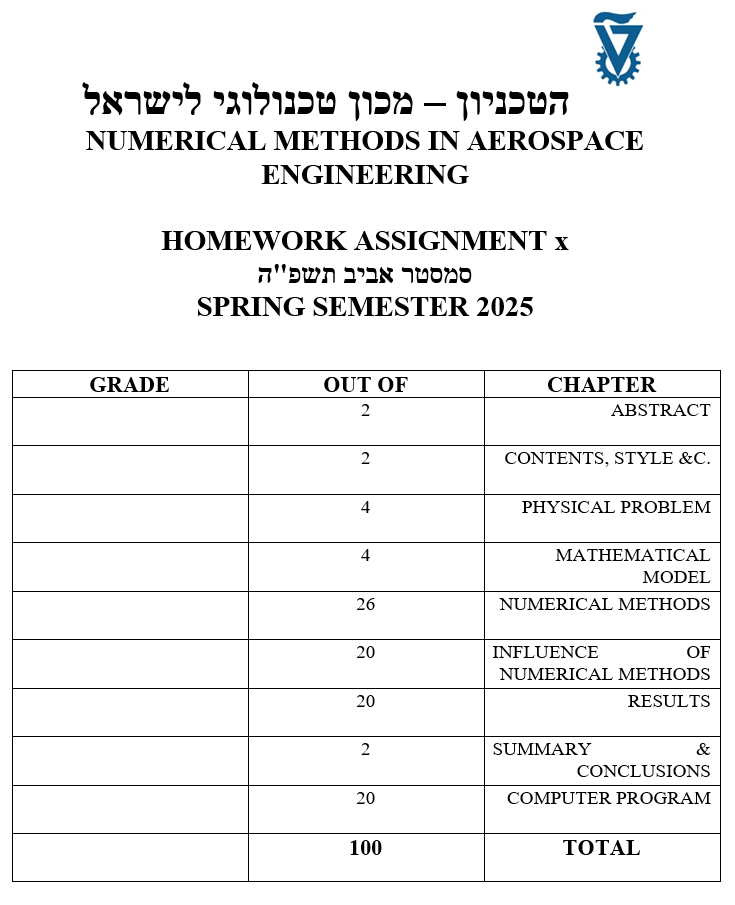
\includegraphics[width=\textwidth]{./../../Cover page for computational assignments 2025.png}
    \label{fig: cover page}
\end{figure}
% \maketitle
\begin{center}
    \Huge
    Almog Dobrescu \qquad ID 214254252 \\ \vspace{0.5cm}
    \today
\end{center}
\newpage

\pagenumbering{roman}
% \setcounter{page}{1}
\begin{abstract}
    hii
\end{abstract}

\tableofcontents
\vfil
\listoffigures
\vfil
\lstlistoflistings
\newpage

\printnomenclature
\newpage

\pagestyle{fancy}
\pagenumbering{arabic}
\setcounter{page}{1}

\section{The Physical Problem}
An incompressible viscose Newtonian fluid flows in a channel.
\begin{figure}[H]
    \centering
    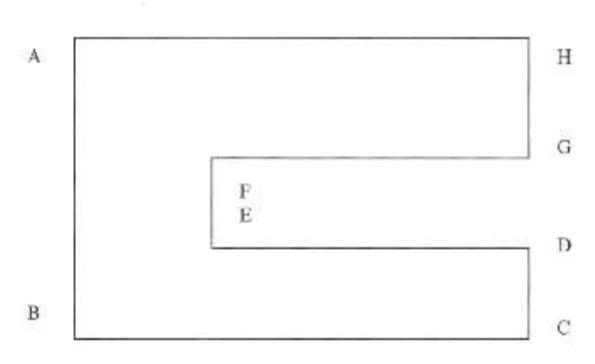
\includegraphics[width=0.7\textwidth]{images/The channel.png}
    \caption{The Channel}
    \label{fig: The Channel}
\end{figure}
Where:
\begin{multicols}{2}
    \begin{itemize}
        \item $AB=12\left[in\right]$
        \item $BC=12\left[in\right]$
        \item $CD=2\left[in\right]$
        \item $DE=6\left[in\right]$
        \item $EF=6\left[in\right]$
        \item $FG=6\left[in\right]$
        \item $GH=4\left[in\right]$
        \item $HA=12\left[in\right]$
    \end{itemize}
\end{multicols}

\section{The Mathematical Model}
The steady-state velocity of the fluid is given by:
\begin{equation}
    \parder{^2\phi}{x^2}+\parder{^2\phi}{y^2}=-\frac{c}{\mu}
    \nomenclature{$c$}{pressure gradient on the flow in a section}
    \nomenclature{$\mu$}{viscosity of the fluid}
\end{equation}
In our case:
\begin{itemize}
    \item $c=0.0002\left[\frac{lb}{in^3}\right]$
    \item $\mu=0.25\cdot10^{-5}\left[\frac{lb\cdot sec}{in^2}\right]$
\end{itemize}
\subsection{Boundary Conditions}
Since the flow is viscose, the boundary conditions are no penetration and no slip. The flow is at steady state so the only direction of the flow is normal the sectional area (outside the paper). Hence the velocity at the boundaries is:
\begin{equation}
    \left.\psi\right|_{AB}=\left.\psi\right|_{BC}=\left.\psi\right|_{CD}=\left.\psi\right|_{DE}=\left.\psi\right|_{EF}=\left.\psi\right|_{FG}=\left.\psi\right|_{GH}=\left.\psi\right|_{HA}=0
\end{equation}


\section{The Numerical Methods}
\subsection{Finite Differencing}
\subsection{Stability Analysis}
\subsection{Convergence Criteria}

\section{Influence of The Numerical Methods}
\subsection{Influence of Number of Elements N}
\subsection{Influence of Convergence Criteria $\varepsilon$}
\subsection{Influence of The Numerical Parameter R}

\section{Results and Discussion}
\label{sec: results and discussion}

\section{Summary and Conclusion}

\newpage
\appendix
\section{Listing of The Computer Program}
\subsection{Parameters}
% \begin{lstinputlisting}[captionpos=b,stringstyle=\color{magenta},frame=single, numbers=left, style=MatLab-editor, basicstyle=\mlttfamily\small, caption={Parameters file},mlshowsectionrules=true]{./matlab/parameters.m}
% \end{lstinputlisting}

\subsection{Main Code}
% \begin{lstinputlisting}[captionpos=b,stringstyle=\color{magenta},frame=single, numbers=left, style=MatLab-editor, basicstyle=\mlttfamily\small, caption={The main file},mlshowsectionrules=true]{./matlab/NM_hw2_CA.m}
% \end{lstinputlisting}

\end{document}